\documentclass{report}

\usepackage[warn]{mathtext}
\usepackage[T2A]{fontenc}
\usepackage[utf8]{luainputenc}
\usepackage[english, russian]{babel}
\usepackage[pdftex]{hyperref}
\usepackage{tempora}
\usepackage[12pt]{extsizes}
\usepackage{listings}
\usepackage{color}
\usepackage{geometry}
\usepackage{enumitem}
\usepackage{multirow}
\usepackage{graphicx}
\usepackage{indentfirst}
\usepackage{amsmath}
\usepackage{wrapfig}
\usepackage{float}

\graphicspath{ {./modules/task_1/ivanov_arkady_rbms/images/} }

\geometry{a4paper,top=2cm,bottom=2cm,left=2.5cm,right=1.5cm}
\setlength{\parskip}{0.5cm}
\setlist{nolistsep, itemsep=0.3cm,parsep=0pt}

\usepackage{listings}
\lstset{language=C++,
        basicstyle=\footnotesize,
		keywordstyle=\color{blue}\ttfamily,
		stringstyle=\color{red}\ttfamily,
		commentstyle=\color{green}\ttfamily,
		morecomment=[l][\color{red}]{\#},
		tabsize=4,
		breaklines=true,
  		breakatwhitespace=true,
  		title=\lstname,
}

\makeatletter
\renewcommand\@biblabel[1]{#1.\hfil}
\makeatother

\begin{document}

\begin{titlepage}

\begin{center}
Министерство науки и высшего образования Российской Федерации
\end{center}

\begin{center}
Федеральное государственное автономное образовательное учреждение высшего образования \\
Национальный исследовательский Нижегородский государственный университет им. Н. И. Лобачевского
\end{center}

\begin{center}
Институт информационных технологий, математики и механики
\end{center}

\vspace{4em}

\begin{center}
\textbf{\LargeОтчет по лабораторной работе} \\
\end{center}
\begin{center}
\textbf{\Large«Поразрядная сортировка для целых чисел с четно-нечетным слиянием Бэтчера»} \\
\end{center}

\vspace{4em}

\newbox{\lbox}
\savebox{\lbox}{\hbox{text}}
\newlength{\maxl}
\setlength{\maxl}{\wd\lbox}
\hfill\parbox{7cm}{
\hspace*{5cm}\hspace*{-5cm}\textbf{Выполнил:}
\\ студент группы 381908-1
\\ Иванов А. А.
\\\\
\hspace*{5cm}\hspace*{-5cm}\textbf{Проверил:}
\\ доцент кафедры МОСТ,
\\ кандидат технических наук
\\ Сысоев А. В.\\
}
\vspace{\fill}

\begin{center} Нижний Новгород \\ 2022 \end{center}

\end{titlepage}

\setcounter{page}{2}

% Содержание
\tableofcontents
\newpage

% Введение
\section*{Введение}
\addcontentsline{toc}{section}{Введение}
\par Задача сортировки в вычислительных алгоритмах встречается нередко. В свою очередь, современные вычислительные системы являются многопроцессорными, что позволяет выполнять вычисления параллельно. А значит можно попытаться распараллелить алгоритм сортировки в целях уменьшения времени вычислений, что является существенным фактором в современных приложениях.
\newpage

% Постановка задачи
\section*{Постановка задачи}
\addcontentsline{toc}{section}{Постановка задачи}
\par Необходимо реализовать последовательную и параллельную версию алгоритма поразрядной сортировки для целых чисел с четно-нечетным слиянием Бэтчера, проверить алгоритм на корректность при помощи системы Google Testing Framework, провести вычислительные эксперименты, сравнить эффективность, сделать выводы. Параллельная реализация алгоритма должна быть выполнена при помощи технологий OpenMP, Intel TBB, std::thread.
\newpage

% Описание алгоритма
\section*{Описание алгоритма}
\addcontentsline{toc}{section}{Описание алгоритма}
\par Алгоритм условно можно разделить на 2 части: сортировку и реализацию обменной сети сортировки Бэтчера. В первой части исходный массив данных делится на блоки равного размера, которые распределяются по потокам, в каждом из которых сортируются поразрядно. Затем потоки организуют реализацию обменной сети сортировки Бэтчера, по мере прохождения которой будет формироваться окончательный отсортированный массив 
\par В параллельной версии алгоритма исходный массив делится на блоки элементов. Блоки должны быть одинакового размера, что является требованием для обменной сети Бэтчера. Количество блоков равняется числу потоков, которые будут производить вычисления. В первой части потоки выполняют поразрядную сортировку выделенных им блоков, затем идет второй шаг: реализация обменной сети, в результате выполнения которой получится отсортированный массив.
\par В последовательной же версии обменную сеть сортировки можно пропустить, поскольку ее реализация на одном потоке не имеет смысла и будет только тормозить алгоритм.

\newpage

% Поразрядная сортировка
\section*{Поразрядная сортировка}
\addcontentsline{toc}{section}{Поразрядная сортировка}
\par В любой системе счисления число можно поделить на разряды и значения, которые эти разряды могут принять. Например число 123 в десятичной системе счисления будет также равно 123 с возможными значениями разряда от 0 до 9, в двоичной оно будет равно 1111011 с возможными значениями разряда 0 или 1. В реальной жизни количество разрядов может быть любым, однако для компьютера, базовые элементы которого строго определены, это не так. Например, 32-битное число можно представить как 32 разряда со значениями от 0 или 1. Или как 4 разряда со значениями от 0 до 255. Второй способ при реализации поразрядной сортировки будет предпочтительнее поскольку в оперативной памяти компьютера данные хранятся побайтово, а не побитно.
\par Итак, предположим, что есть массив 4-байтных чисел, в которых каждый разряд может принимать значения от 0 до 255. Для начала необходимо создать массив счетчиков для каждого разряда, проинициализированный нулями. Размер этого массива будет равен 4*256, что равняется количеству разрядов числа * количество возможных значений разряда. Затем исходный массив проходится побайтово и соответствующее значение для соответствующего разряда в массиве счетчиков увеличивается на единицу. Затем для каждого разряда в массиве счетчиков производится следующая операция: первый элемент заменяется на 0, а остальные становятся суммой предыдущего значения счетчиков и суммы всех пройденных до этого элементов счетчика. Это необходимо для того, чтобы сформировать смещения для элементов исходного массива при сортировке.
\par Затем идет этап сортировки: для каждого разряда, начиная с младшего и заканчивая старшим, берется массив счетчиков соответствующего разряда и элементы исходного массива перегруппируются в соответствии со значениями элементов счетчика (смещения). В результате получится отсортированный массив.

\newpage

% Четно-нечетное слияние Бэтчера
\section*{Четно-нечетное слияние Бэтчера}
\addcontentsline{toc}{section}{Четно-нечетное слияние Бэтчера}
\par Четно-нечетное слияние бетчера представляет собой реализацию сортировочной сети, суть которой заключается в реализации выполнения операции компаратора между отсортированными блоками данных одинакового размера. Операция компаратора выполняется для двух блоков и заключается в том, что для одного из двух блоков, участвующих в операции, остаются наименьшие элементы из них в порядке возрастания, а для другого - наибольшие элементы, но также в порядке возрастания. Количество этих элементов равняется размеру блока. Исходный блок заменяется полученным результатом и используется в дальнейших операциях компаратора.

\newpage

% Описание схемы распараллеливания
\section*{Описание схемы распараллеливания}
\addcontentsline{toc}{section}{Описание схемы распараллеливания}
\par Распараллеливание происходит за счет разбиения исходного массива на блоки данных, распределения их по потокам, которые параллельно реализуют алгоритм поразрядной сортировки, а затем выполняют проход по обменной сети сортировки Бэтчера. Код был написан таким образом, что реализация OpenMP, TBB, std::thread отличаются друг от друга только тем, что в TBB и std::thread используется собственный класс барьера для потоков, а не встроенная реализация, как в OpenMP. Сделано это было для того, чтобы не переписывать код несколько раз, а также гарантировать правильность работы алгоритма. В данном алгоритме нежелательно позволять распределять данные библиотекам, поскольку должно гарантироваться деление исходного массива на блоки одинакового размера. Также, количество запущенных потоков также должно быть строго определено, чтобы не было возможности появления ситуации взаимоблокировки потоков, которая может появиться на барьерах, которые используются при реализации обменной сортировочной сети.

\newpage

% Описание программной реализации
\section*{Описание программной реализации}
\addcontentsline{toc}{section}{Описание программной реализации}
\par Программа состоит из заголовочных файлов Barrier.h, serviceFunctions.h, rbms.h, а также двух файлов исходного кода main.cpp и rbms.cpp
\par В заголовочном файле Barrier.h содержится класс барьера, предназначенного для синхронизации потоков, подошедших к нему: потоки останавливаются на барьере до тех пор, пока заданное количество не окажется у барьера. Состоит из конструктора инициализации и метода ожидания:
\begin{lstlisting}
explicit Barrier(unsigned int n)
void wait()
\end{lstlisting}
\par В заголовочном файле serviceFunctions.h содержатся шаблоны функций, выполняющих вспомогательные операции при использовании программы: получение случайного значения в заданном интервале, заполнение массива случайными значениями в заданном интервале, проверка на строгое возрастание/убывание, заполнение массива строгим возрастанием/убыванием, вывод массива в консоль, проверка на нестрогое возрастание, проверка равенства двух массивов
\begin{lstlisting}
template<class T>
T getRandValue(T from, T to)

template<class T>
void fillVecWithRandValues(T* data, int size, T from, T to)

template<class T>
bool isStrictAscending(T* data, int size, T startValue)

template<class T>
bool isStrictDescending(T* data, int size, T startValue)

template<class T>
void fillStrictAscending(T* data, int size, T startValue)

template<class T>
void fillStrictDescending(T* data, int size, T startValue)

template<class T>
void printVector(const std::vector<T>& vec)

template<class T>
bool isAscending(T* data, int size)

template<class T>
bool isVecSame(const std::vector<T>& v1, const std::vector<T>& v2)
\end{lstlisting}
\par В заголовочном файле rbms.h содержатся шаблоны функций: поразрядной сортировки, поразрядной сортировки с четно-нечетным слиянием Бэтчера в реализациях OpenMP, TBB и std::thread, вспомогательные для них функции-шаблоны, а также прототип функции, которая используется при вычислении партнера при реализации обменной сети Бэтчера. Кроме того есть макроc USE\_THREAD\_AFFINITY, при помощи которого можно указать, будет ли использоваться механизм привязки потоков к ядрам. Механизм привязки доступен только для системы под управлением OS Windows
\begin{lstlisting}
int partner(int nodeIndex, int mergeStage, int mergeStageStep);

template <class T>
std::vector<int> createAndPrepareCounters(std::vector<T>* data, int offset, int count)

template<class T>
void radixSort(std::vector<T>* data, int offset, int count)

template<class T>
void mergeFragments(T* data, T* res, T* partnerData,
    int blockSize, int selfID, int partnerID) {
    
template<class T>
void radixBatchersMergesort_omp(std::vector<T>* data, int degree)

template<class T>
void radixBatchersMergesort_tbb(std::vector<T>* data, int degree)

template<class T>
void singleThreadComputing(int selfID, Barrier* b1, Barrier* b2, Barrier* b3,
    T** from, T** to, std::vector<T>* data, int blockSize,
    int degree, T* mainData)
    
template<class T>
void radixBatchersMergesort_std(std::vector<T>* data, int degree)
\end{lstlisting}
\par В файле rbms.cpp содержится реализация функции, которая используется при вычислении партнера при реализации обменной сети Бэтчера, а в файле main.cpp: шаблоны функций, использующихся для проверки корректности алгоритмов сортировки, а также тесты для системы Google Testing Framework

\newpage

% Подтверждение корректности
\section*{Подтверждение корректности}
\addcontentsline{toc}{section}{Подтверждение корректности}
Для подтверждения корректности использовался фреймворк Google Testing Framework, при помощи которого тестировались различные возможные варианты использования алгоритмов. Тестирование заключалось в проверке как алгоритма поразрядной сортировки, так и всего алгоритма в целом. Успешное прохождение всех тестов подтверждает корректность работы программы.
\newpage

% Результаты экспериментов
\section*{Результаты экспериментов}
\addcontentsline{toc}{section}{Результаты экспериментов}
Вычислительные эксперименты для оценки эффективности работы параллельных алгоритмов проводились на ПК со следующими характеристиками:
\begin{itemize}
    \item Процессор: AMD Ryzen 7 3700X, 3.60-4.40 ГГц, 8 ядер, 16 потоков;
    \item Оперативная память: 16 ГБ, DDR4, 3600 МГц, CL16;
    \item Операционная система: Windows 10 Pro.
\end{itemize}
\par Был проведен эксперимент, в котором производилось измерение ускорения вычислений относительно одного потока для различных реализаций с различным количеством элементов в исходном массиве. Ось абсцисс показывает степень, в которую возводится число 10, результат будет количеством элементов в массиве. Ось ординат показывает ускорение вычислений относительно одного потока
\begin{figure}[H]
    \centering
    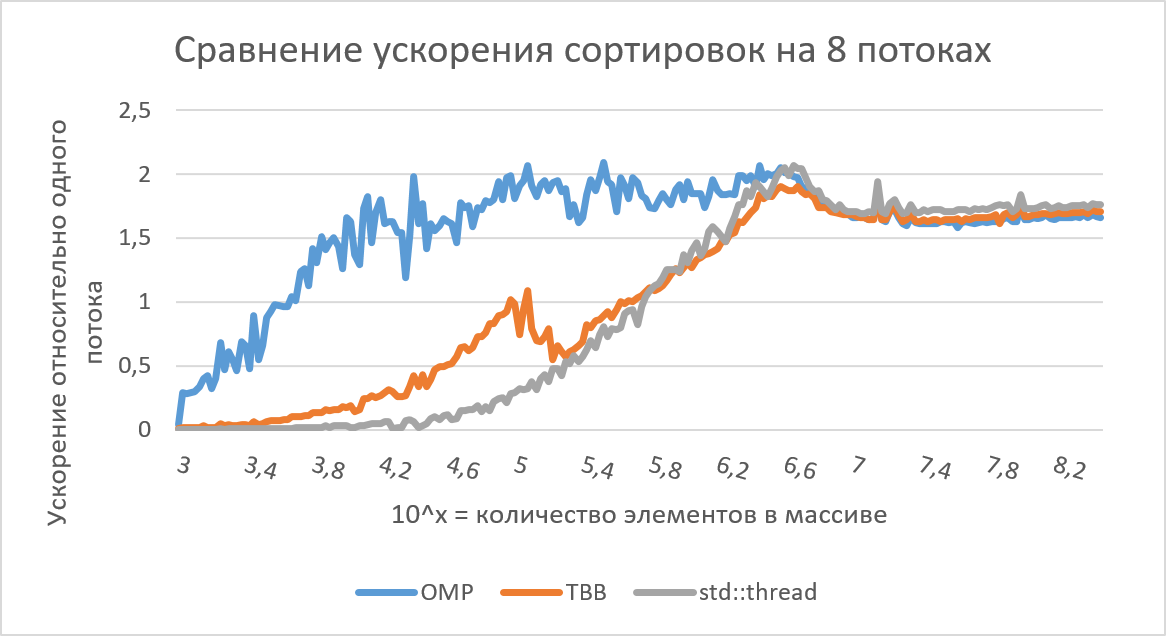
\includegraphics[width=0.85\textwidth]{boost_comparsion_8thrd.png}
    \caption{Сравнение ускорения реализаций сортировок}
    \label{fig:my_label_1}
\end{figure}
\par Был проведен эксперимент, в котором производилось измерение времени выполнения вычислений относительно одного потока для различных реализаций с различным количеством элементов в исходном массиве.
\begin{figure}[H]
    \centering
    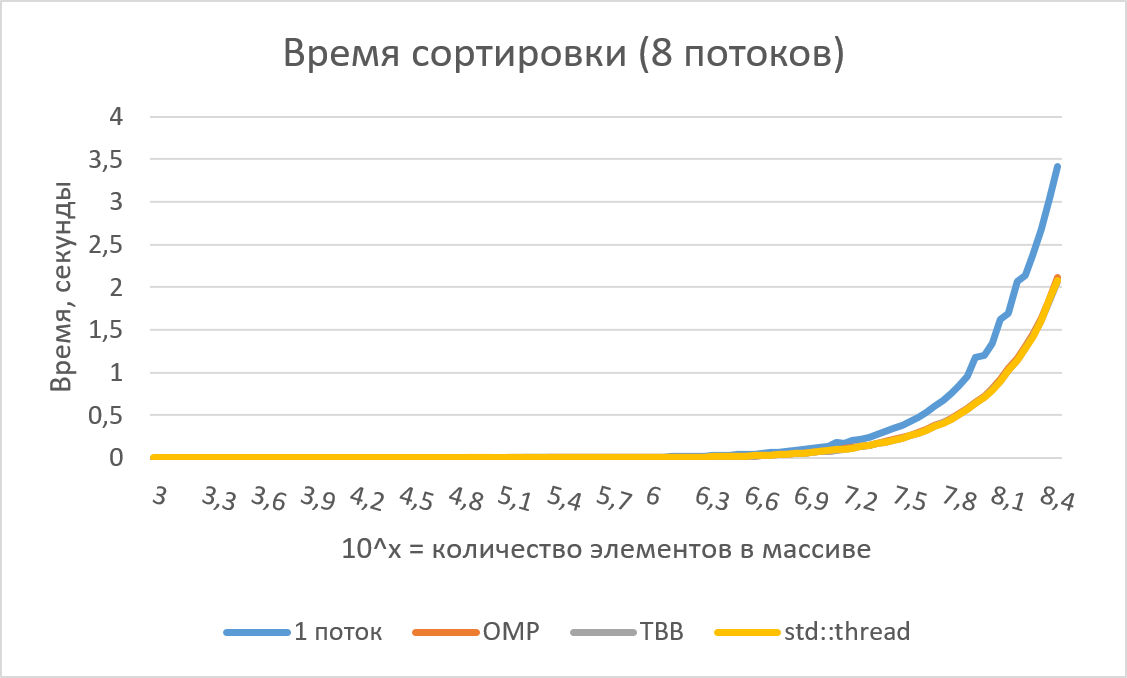
\includegraphics[width=0.85\textwidth]{sort_time_8thrd.png}
    \caption{Сравнение времени выполнения вычислений}
    \label{fig:my_label_2}
\end{figure}
\par Был проведен эксперимент, в котором производилось измерение ускорения для реализации OpenMP на разном количестве исходных данных и на различных количествах потоков.
\begin{figure}[H]
    \centering
    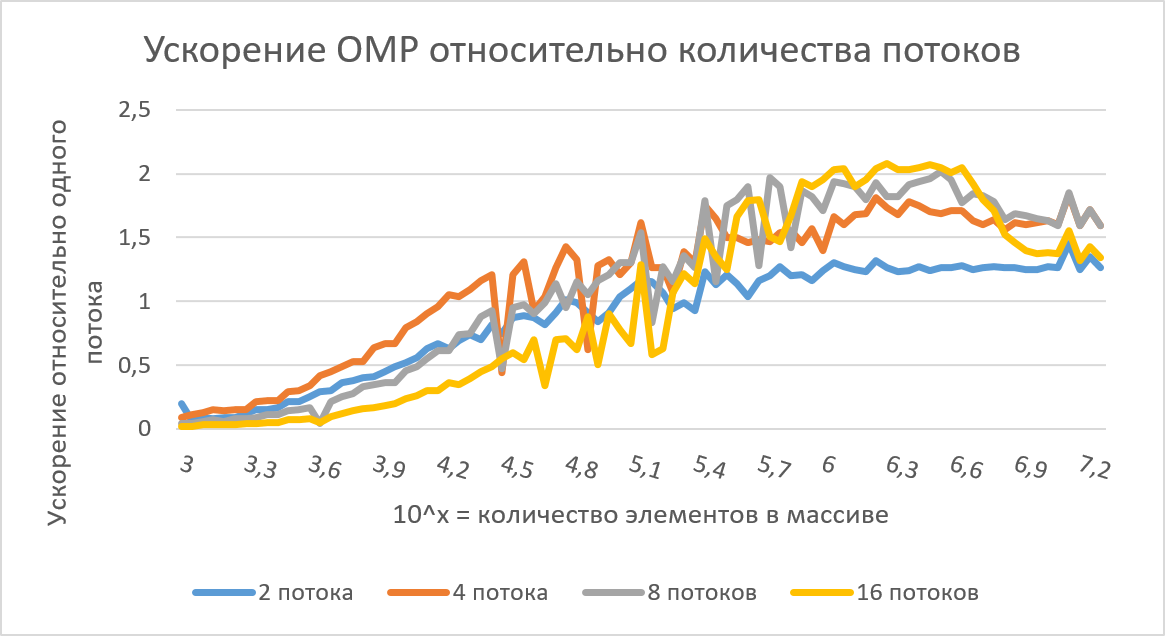
\includegraphics[width=0.85\textwidth]{boost_omp.png}
    \caption{Сравнение ускорения для OpenMP реализации}
    \label{fig:my_label_3}
\end{figure}
\par Был проведен эксперимент, в котором производилось измерение ускорения для реализации TBB на разном количестве исходных данных и на различных количествах потоков.
\begin{figure}[H]
    \centering
    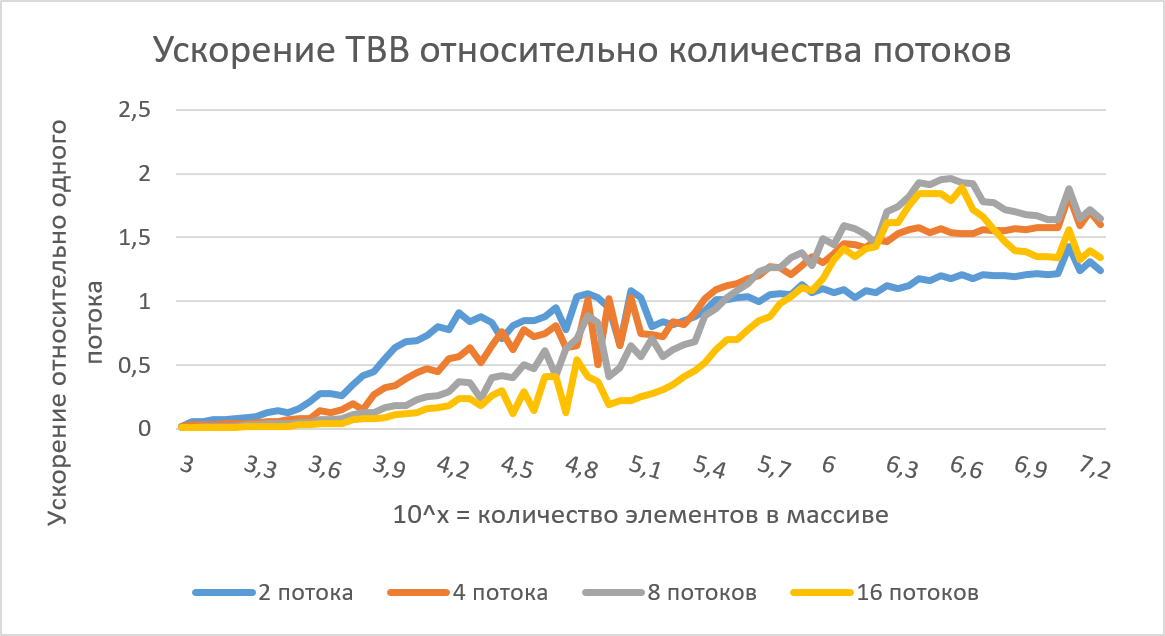
\includegraphics[width=0.85\textwidth]{boost_tbb.png}
    \caption{Сравнение ускорения для TBB реализации}
    \label{fig:my_label_4}
\end{figure}
\par Был проведен эксперимент, в котором производилось измерение ускорения для реализации std::thread на разном количестве исходных данных и на различных количествах потоков без использования механизма привязки потоков к ядрам
\begin{figure}[H]
    \centering
    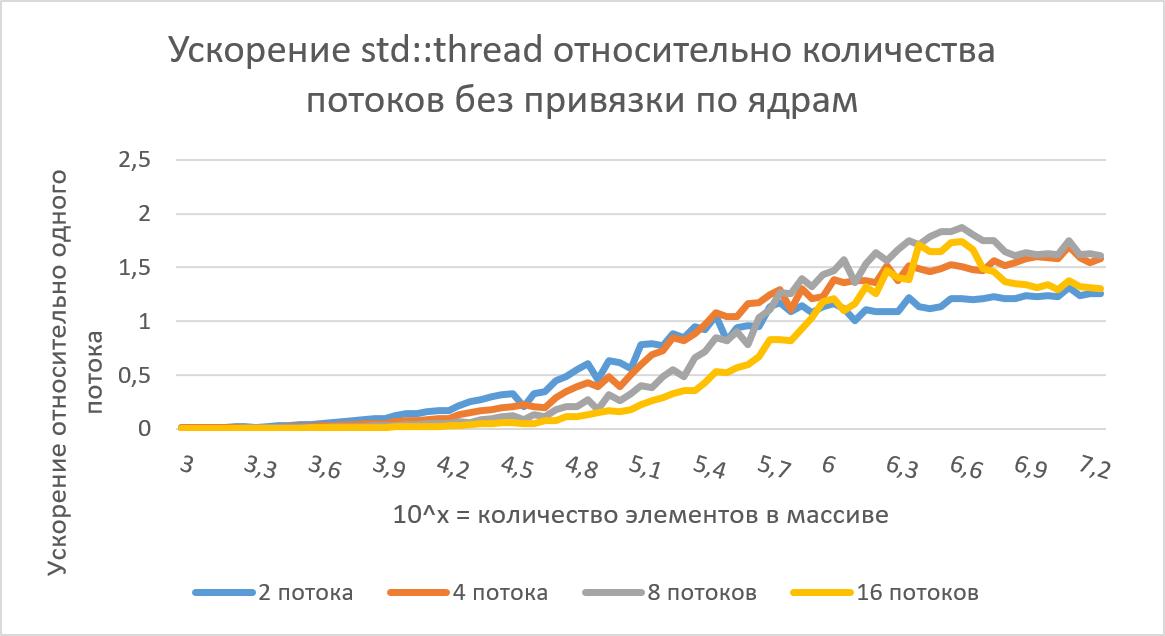
\includegraphics[width=0.85\textwidth]{boost_std_without_affinity.png}
    \caption{Сравнение ускорения для std::thread реализации без привязки по ядрам}
    \label{fig:my_label_5}
\end{figure}
\par Был проведен эксперимент, в котором производилось измерение ускорения для реализации std::thread на разном количестве исходных данных и на различных количествах потоков с использованием механизма привязки потоков к ядрам
\begin{figure}[H]
    \centering
    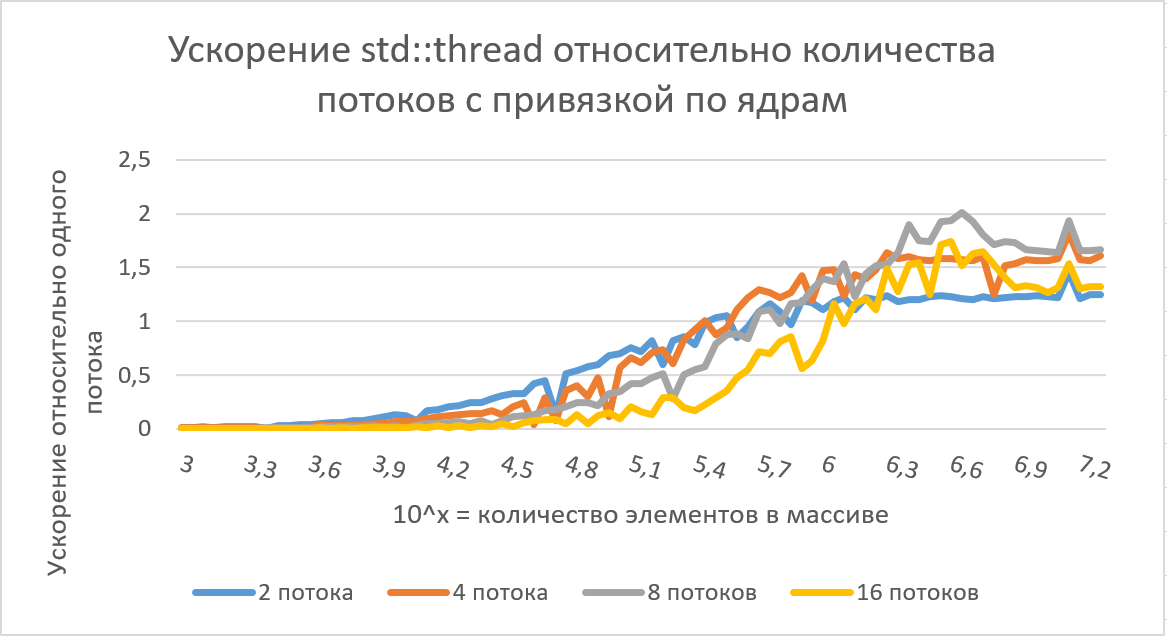
\includegraphics[width=0.85\textwidth]{boost_std_with_affinity.png}
    \caption{Сравнение ускорения для std::thread реализации с привязкой по ядрам}
    \label{fig:my_label_6}
\end{figure}

\newpage

% Выводы из результатов экспериментов
\section*{Выводы из результатов экспериментов}
\addcontentsline{toc}{section}{Выводы из результатов экспериментов}
\par Из результатов экспериментов можно сделать следующие выводы:
\begin{itemize}
    \item OpenMP реализация на восьми потоках показывает ускорение параллельной версии относительно последовательной начиная с 4500 элементов, TBB и std::thread - с 500 тыс. элементов. 
    \item OpenMP реализия на восьми потоках показывает большее ускорение относительно TBB и std::thread когда количество сортируемых элементов меньше 375 тыс. Скорее всего, связано это с тем, что OpenMP может замораживать потоки до востребования, а не завершать их как только параллельная часть алгоритма закончена. На создание потоков тратится время, которое при малом количестве сортируемых элементов может быть значительным относительно времени сортировки.
    \item std::thread релазиция на восьми потоках с их привязкой по ядрам показывает незначительно, но большее ускорение, чем TBB и OpenMP когда количество сортируемых элементов является больше 375 тыс. Скорее всего, связано это с тем, что привязка потоков к ядрам позволяет более эффективно использовать кеш центрального процессора, ведь если поток будет непривязан ни к одному ядру, то кеш будет постоянно перезагружаться, когда поток будет мигрировать с одного ядра на другое, что в свою очередь будет вносить задержки.
    \item Начиная с 10 млн. элементов, ускорение для всех реализованных параллельных алгоритмах сортировок на 8 потоках перестает расти либо рост становится незначительным и держится в райноне 1.7
    \item Наибольшую эффективность на 8 потоках показывают алгоритмы, когда колиечство элементов равно 375 тыс. Наибольшее ускорение при этом показывает std::thread с показателем в 2.04
    \item OpenMP реализация на разном количестве потоков и разном размере исходных данных показывает различные ускорения. До 20 тыс. элементов эффективнее всего будет использовать один поток (просто поразрядная сортировка). От 20 тыс. элементов до 280 тыс. наибольшую эффективность показывают 4 потока. От 280 тыс. до 1 млн. - 8 потоков. От 1 млн. до 5 млн. - 16 потоков. От 5 млн. - 8 потоков
    \item TBB реализация на разном количестве потоков и разном размере исходных данных показывает различные ускорения, однако эффективным можно считать лишь тот участок, в котором ускорение больше единцы и на данном участке наиболшее ускорение показывают 8 потоков. Начинается этот участок с 400 тыс. элементов. Те же результаты показывает std::thread.
    \item std::thread реализция с привязкой потоков по ядрам показывает немного большее ускорение, чем без привязки по ядрам.
\end{itemize}

\newpage

% Заключение
\section*{Заключение}
\addcontentsline{toc}{section}{Заключение}
\par В ходе выполнения данной лабораторной работы были реализованы последовательная версия алгоритма и параллельные версии с использованием технологий OpenMP, TBB и std::thread, была доказана корректность их работы, были проведены эксперименты, общим итогом которых можно сказать, что универсального алгоритма, показывающего эффективность на всем множестве возможных значений количества исходных данных, нет, а для достижения максимальной эффективности необходимо знать размер сортируемого массива и выбирать алгоритм, показывающий наибольшее ускорение на данном размере. 

\newpage

% Литература
\section*{Литература}
\addcontentsline{toc}{section}{Литература}
\begin{enumerate}
    \item Хабр. Сеть обменной сортировки со слиянием Бэтчера - Электронный ресурс. URL: \newline
    \url{https://habr.com/ru/post/275889/}
    \item Алголист. Поразрядная сортировка - Элеметронный ресурс. URL: \newline
    \url{https://algolist.manual.ru/sort/radix_sort.php}
    \item Sparky Dots. Batcher's odd-even merging network - Электронный ресурс. URL: \newline
    \url{https://sparkydots.blogspot.com/2015/05/batchers-odd-even-merging-network.html}
    \item Хабр. Создание барьера синхронизации с использованием C++11 - Электронный ресурс. URL: \newline
    \url{https://habr.com/ru/post/246947/}
    \item Хабр. Потоки, блокировки и условные переменные в C++11 [Часть 2] - Электронный ресурс. URL: \newline
    \url{https://habr.com/ru/post/182626/}
\end{enumerate}
\newpage

% Приложение
\section*{Приложение}
\addcontentsline{toc}{section}{Приложение}
Barrier.h
\begin{lstlisting}
// Copyright 2022 Ivanov Arkady
#ifndef MODULES_TASK_3_IVANOV_REPORT_BARRIER_H_
#define MODULES_TASK_3_IVANOV_REPORT_BARRIER_H_

#include <condition_variable>  // NOLINT [build/c++11]
#include <mutex>  // NOLINT [build/c++11]

/*
* Barrier class
* In parallel code can't be called sequentially
* or there will be a possibility of a deadlock +
* barrier crossing of single thread
* NOT TO DO: {
*       // work
*       barrier.wait();
*       // work
*       barrier.wait();
* }
*
* insted use 2 alternating barriers: {
*       // work
*       barrier1.wait();
*       // work
*       barrier2.wait();
*       // work
*       barrier1.wait();
*       // work
*       barrier2.wait();
*       // etc
* }
*/
class Barrier {
private:
    const unsigned int threadCount;
    volatile unsigned int threadsWaiting;
    std::condition_variable waitVariable;
    std::mutex mutex;
    volatile bool isLocked;

public:
    Barrier() = delete;
    Barrier(const Barrier& c) = delete;
    Barrier& operator=(const Barrier& c) = delete;

    explicit Barrier(unsigned int n) :
        threadCount(n),
        threadsWaiting(0),
        isLocked(true) {}


    void wait() {
        std::unique_lock<std::mutex> lk(mutex);
        ++threadsWaiting;
        if (threadsWaiting >= threadCount) {
            threadsWaiting = 0;
            isLocked = false;

            lk.unlock();
            waitVariable.notify_all();
        } else {
            while (isLocked && threadsWaiting != 0)
                waitVariable.wait(lk);
            isLocked = true;  // to make reusable
        }
    }
};
#endif  // MODULES_TASK_3_IVANOV_REPORT_BARRIER_H_
\end{lstlisting}
serviceFunctions.h
\begin{lstlisting}
// Copyright 2022 Ivanov Arkady
#ifndef MODULES_TASK_3_IVANOV_REPORT_SERVICEFUNCTIONS_H_
#define MODULES_TASK_3_IVANOV_REPORT_SERVICEFUNCTIONS_H_

#include <vector>
#include <random>
#include <algorithm>
#include <utility>
#include <iostream>


template<class T>
T getRandValue(T from, T to) {
    static std::random_device rd;
    static std::mt19937 gen(rd());
    std::uniform_int_distribution<T> dist(from, to);
    return dist(gen);
}

template<class T>
void fillVecWithRandValues(T* data, int size, T from, T to) {
    static std::random_device rd;
    static std::mt19937 gen(rd());
    std::uniform_int_distribution<T> dist(from, to);
    for (int i = 0; i < size; i++) {
        data[i] = dist(gen);
    }
}

template<class T>
bool isStrictAscending(T* data, int size, T startValue) {
    for (int i = 0; i < size; i++)
        if (data[i] != startValue++)
            return false;
    return true;
}

template<class T>
bool isStrictDescending(T* data, int size, T startValue) {
    for (int i = 0; i < size; i++)
        if (data[i] != startValue--)
            return false;
    return true;
}

template<class T>
void fillStrictAscending(T* data, int size, T startValue) {
    for (int i = 0; i < size; i++)
        data[i] = startValue++;
}

template<class T>
void fillStrictDescending(T* data, int size, T startValue) {
    for (int i = 0; i < size; i++)
        data[i] = startValue--;
}

template<class T>
void printVector(const std::vector<T>& vec) {
    for (int i = 0; i < vec.size(); i++)
        std::cout << vec[i] << " ";
    std::cout << std::endl;
}

template<class T>
bool isAscending(T* data, int size) {
    for (int i = 1; i < size; i++) {
        if (data[i - 1] > data[i])
            return false;
    }
    return true;
}

template<class T>
bool isVecSame(const std::vector<T>& v1, const std::vector<T>& v2) {
    if (v1.size() != v2.size())
        return false;
    for (size_t i = 0; i < v1.size(); i++)
        if (v1[i] != v2[i])
            return false;
    return true;
}
#endif  // MODULES_TASK_3_IVANOV_REPORT_SERVICEFUNCTIONS_H_
\end{lstlisting}
rbms.h
\begin{lstlisting}
// Copyright 2022 Ivanov Arkady
#ifndef MODULES_TASK_3_IVANOV_REPORT_RBMS_H_
#define MODULES_TASK_3_IVANOV_REPORT_RBMS_H_

#define USE_THREAD_AFFINITY 0

#include <stdint.h>
#include <tbb/task_scheduler_init.h>
#include <tbb/task_group.h>

#if WIN32 == 1 && USE_THREAD_AFFINITY == 1
#include <Windows.h>
#endif  // WIN32 == 1 && USE_EFFICIENCY_TESTS == 1

#include <omp.h>
#include "Barrier.h"
#include "serviceFunctions.h"

#include <thread>  // NOLINT [build/c++11]


int partner(int nodeIndex, int mergeStage, int mergeStageStep);

// <RadixSort>
template <class T>
std::vector<int> createAndPrepareCounters(std::vector<T>* data, int offset, int count) {
    std::vector<int> counters(256 * sizeof(T));
    std::fill_n(counters.data(), counters.size(), 0);
    unsigned char* start = reinterpret_cast<unsigned char*>(
        data->data() + offset);
    unsigned char* stop = reinterpret_cast<unsigned char*>(
        data->data() + offset + count);

    while (start != stop) {
        for (int i = 0; i < static_cast<int>(sizeof(T)); i++) {
            counters[*start + 256 * i]++;
            start++;
        }
    }

    for (int i = 0; i < static_cast<int>(sizeof(T)); i++) {
        int sum = 0;
        if (counters[256 * i] == count)
            continue;
        for (int j = 0; j < 256; j++) {
            int tmp = counters[256 * i + j];
            counters[256 * i + j] = sum;
            sum += tmp;
        }
    }
    return counters;
}

template<class T>
void radixSort(std::vector<T>* data, int offset, int count) {
    std::vector<int> counters =
        createAndPrepareCounters(data, offset, count);

    std::vector<T> res(count);
    int j;
    for (j = 0; j < static_cast<int>(sizeof(T)); j++) {
        int* countersPtr = counters.data() + 256 * j;
        if (*countersPtr == count)
            break;

        T* dPtr, * rPtr;
        unsigned char* dataPtr;
        if (j % 2 == 0) {
            dPtr = data->data() + offset;
            dataPtr = reinterpret_cast<unsigned char*>(
                data->data() + offset);
            rPtr = res.data();
        } else {
            dPtr = res.data();
            dataPtr = reinterpret_cast<unsigned char*>(res.data());
            rPtr = data->data() + offset;
        }
        dataPtr += j;

        for (int i = 0; i < count; i++) {
            rPtr[*(countersPtr + *dataPtr)] = dPtr[i];
            *(countersPtr + *dataPtr) = *(countersPtr + *dataPtr) + 1;
            dataPtr += sizeof(T);
        }
    }

    if (j % 2 == 1) {
        for (int i = 0; i < count; i++)
            data->operator[](i + offset) = res[i];
    }
}
// </RadixSort>

// <ComparatorFunction>
template<class T>
void mergeFragments(T* data, T* res, T* partnerData,
    int blockSize, int selfID, int partnerID) {
    if (selfID == partnerID)
        return;

    bool isLeft = selfID < partnerID;

    if (isLeft) {
        T* firstPtr = data;
        int usedFirst = 0;

        T* secondPtr = partnerData;
        int usedSecond = 0;

        for (int i = 0; i < blockSize; i++) {
            if (usedFirst < blockSize && usedSecond < blockSize) {
                if (*firstPtr < *secondPtr) {
                    res[i] = *firstPtr;
                    firstPtr++;
                    usedFirst++;
                } else {
                    res[i] = *secondPtr;
                    secondPtr++;
                    usedSecond++;
                }
            } else if (usedFirst < blockSize && usedSecond >= blockSize) {
                res[i] = *firstPtr;
                firstPtr++;
                usedFirst++;
            } else if (usedFirst >= blockSize && usedSecond < blockSize) {
                res[i] = *secondPtr;
                secondPtr++;
                usedSecond++;
            } else {
                throw "Impossible exception";
            }
        }
        return;
    }

    // if isLeft = false
    T* firstPtr = data + blockSize - 1;
    int usedFirst = 0;

    T* secondPtr = partnerData + blockSize - 1;
    int usedSecond = 0;

    for (int i = blockSize - 1; i >= 0; i--) {
        if (usedFirst < blockSize && usedSecond < blockSize) {
            if (*firstPtr > *secondPtr) {
                res[i] = *firstPtr;
                firstPtr--;
                usedFirst++;
            } else {
                res[i] = *secondPtr;
                secondPtr--;
                usedSecond++;
            }
        } else if (usedFirst < blockSize && usedSecond >= blockSize) {
            res[i] = *firstPtr;
            firstPtr--;
            usedFirst++;
        } else if (usedFirst >= blockSize && usedSecond < blockSize) {
            res[i] = *secondPtr;
            secondPtr--;
            usedSecond++;
        } else {
            throw "Impossible exception";
        }
    }
}
// </ComparatorFunction>

// <OMP Realisation>
template<class T>
void radixBatchersMergesort_omp(std::vector<T>* data, int degree) {
    if (degree == 0) {  // numThreads = 1
        radixSort<T>(data, 0, data->size());
        return;
    }

    int numThreads = 1 << degree;
    if (numThreads > static_cast<int>(data->size())) {
        radixSort<T>(data, 0, data->size());
        return;
    }

    size_t oldSize = data->size();
    bool isResized = false;
    if (oldSize % numThreads != 0) {
        data->resize(oldSize + (numThreads - oldSize % numThreads), ~0);
        isResized = true;
    }

    int size = data->size();
    int blockSize = size / numThreads;

    std::vector<T> res(size);

    T** from = new T * [numThreads];
    T** to = new T * [numThreads];

    for (int i = 0; i < numThreads; i++) {
        from[i] = data->data() + blockSize * i;
        to[i] = res.data() + blockSize * i;
    }
    T* mainData = data->data();

    #pragma omp parallel num_threads(numThreads)
    {
        int selfID = omp_get_thread_num();
        // sort step
        radixSort<T>(data, selfID * blockSize, blockSize);

        #pragma omp barrier

        // merge step
        // Batcher's merge network realisation
        int partnerID;

        for (int stage = 1; stage <= degree; stage++) {
            for (int step = 1; step <= stage; step++) {
                partnerID = partner(selfID, stage, step);

                mergeFragments(from[selfID], to[selfID], from[partnerID], blockSize, selfID, partnerID);
                #pragma omp barrier

                if (selfID != partnerID)
                    std::swap(from[selfID], to[selfID]);
                #pragma omp barrier

                if (stage == degree && step == degree) {
                    for (int i = 0; i < blockSize; i++)
                        mainData[selfID * blockSize + i] = from[selfID][i];
                }
            }
        }
        #pragma omp barrier
        {}
    }
    delete[] from;
    delete[] to;
    if (isResized)
        data->resize(oldSize);
}
// </OMP Realisation>

// <TBB Realisation>
template<class T>
void radixBatchersMergesort_tbb(std::vector<T>* data, int degree) {
    if (degree == 0) {  // numThreads = 1
        radixSort<T>(data, 0, data->size());
        return;
    }

    int numThreads = 1 << degree;
    if (numThreads > static_cast<int>(data->size())) {
        radixSort<T>(data, 0, data->size());
        return;
    }

    size_t oldSize = data->size();
    bool isResized = false;
    if (oldSize % numThreads != 0) {
        data->resize(oldSize + (numThreads - oldSize % numThreads), ~0);
        isResized = true;
    }

    int size = data->size();
    int blockSize = size / numThreads;

    std::vector<T> res(size);

    T** from = new T * [numThreads];
    T** to = new T * [numThreads];

    for (int i = 0; i < numThreads; i++) {
        from[i] = data->data() + blockSize * i;
        to[i] = res.data() + blockSize * i;
    }
    T* mainData = data->data();


    tbb::task_scheduler_init init(numThreads);
    tbb::task_group group;
    Barrier b1(numThreads), b2(numThreads), b3(numThreads);

    for (int selfID = 0; selfID < numThreads; selfID++) {
        group.run([selfID, &b1, &b2, &b3, from, to, data,
            blockSize, degree, mainData]() {
                // sort step
                radixSort<T>(data, selfID * blockSize, blockSize);

                // barrier
                b3.wait();

                // merge step
                // Batcher's merge network realisation
                int partnerID;

                for (int stage = 1; stage <= degree; stage++) {
                    for (int step = 1; step <= stage; step++) {
                        partnerID = partner(selfID, stage, step);

                        mergeFragments(from[selfID], to[selfID], from[partnerID], blockSize, selfID, partnerID);
                        b1.wait();

                        if (selfID != partnerID)
                            std::swap(from[selfID], to[selfID]);
                        b2.wait();

                        if (stage == degree && step == degree) {
                            for (int i = 0; i < blockSize; i++)
                                mainData[selfID * blockSize + i] = from[selfID][i];
                        }
                    }
                }
                b3.wait();
            });
    }
    group.wait();

    delete[] from;
    delete[] to;

    if (isResized)
        data->resize(oldSize);
}
// </TBB Realisation>

// <STD Realisation>
template<class T>
void singleThreadComputing(int selfID, Barrier* b1, Barrier* b2, Barrier* b3,
    T** from, T** to, std::vector<T>* data, int blockSize,
    int degree, T* mainData) {
    // sort step
    radixSort<T>(data, selfID * blockSize, blockSize);

    // barrier
    b3->wait();

    // merge step
    // Batcher's merge network realisation
    int partnerID;

    for (int stage = 1; stage <= degree; stage++) {
        for (int step = 1; step <= stage; step++) {
            partnerID = partner(selfID, stage, step);

            mergeFragments(from[selfID], to[selfID], from[partnerID], blockSize, selfID, partnerID);
            b1->wait();

            if (selfID != partnerID)
                std::swap(from[selfID], to[selfID]);
            b2->wait();

            if (stage == degree && step == degree) {
                for (int i = 0; i < blockSize; i++)
                    mainData[selfID * blockSize + i] = from[selfID][i];
            }
        }
    }
    b3->wait();
}

template<class T>
void radixBatchersMergesort_std(std::vector<T>* data, int degree) {
    if (degree == 0) {  // numThreads = 1
        radixSort<T>(data, 0, data->size());
        return;
    }

    int numThreads = 1 << degree;
    if (numThreads > static_cast<int>(data->size())) {
        radixSort<T>(data, 0, data->size());
        return;
    }

    size_t oldSize = data->size();
    bool isResized = false;
    if (oldSize % numThreads != 0) {
        data->resize(oldSize + (numThreads - oldSize % numThreads), ~0);
        isResized = true;
    }

    int size = data->size();
    int blockSize = size / numThreads;

    std::vector<T> res(size);

    T** from = new T * [numThreads];
    T** to = new T * [numThreads];

    for (int i = 0; i < numThreads; i++) {
        from[i] = data->data() + blockSize * i;
        to[i] = res.data() + blockSize * i;
    }
    T* mainData = data->data();

    Barrier b1(numThreads), b2(numThreads), b3(numThreads);
    std::vector<std::thread> threads;

    for (int selfID = 0; selfID < numThreads; selfID++) {
        threads.emplace_back(singleThreadComputing<T>,
            selfID, &b1, &b2, &b3,
            from, to, data, blockSize, degree, mainData);

#if WIN32 == 1 && USE_THREAD_AFFINITY == 1
        unsigned int offset;
        if (numThreads <= std::thread::hardware_concurrency() / 2)
            offset = static_cast<unsigned int>(selfID) * 2;
        else
            offset = static_cast<unsigned int>(selfID) % std::thread::hardware_concurrency();

        DWORD_PTR dw = SetThreadAffinityMask(threads.back().native_handle(), DWORD_PTR(1) << offset);
        if (dw == 0) {
            DWORD dwErr = GetLastError();
            std::cerr << "SetThreadAffinityMask fail, GLE = " << dwErr << std::endl;
        }
#endif  // WIN32 == 1 && USE_EFFICIENCY_TESTS == 1
    }

    for (auto& t : threads)
        t.join();

    delete[] from;
    delete[] to;

    if (isResized)
        data->resize(oldSize);
}
// </STD Realisation>
#endif  // MODULES_TASK_3_IVANOV_REPORT_RBMS_H_
\end{lstlisting}
rbms.cpp
\begin{lstlisting}
// Copyright 2022 Ivanov Arkady
#include "../../../modules/task_3/ivanov_report/rbms.h"

int partner(int nodeIndex, int mergeStage, int mergeStageStep) {
    if (mergeStageStep > mergeStage)
        throw "ERROR";

    if (mergeStageStep == 1) {
        return nodeIndex ^ (1 << (mergeStage - 1));
    } else {
        int scale = 1 << (mergeStage - mergeStageStep);  // difference between nodes for stage n stageStep n.s
        int box = 1 << mergeStageStep;
        int sn = nodeIndex / scale - (nodeIndex / scale / box) * box;
        if (sn == 0 || sn == box - 1)
            return nodeIndex;
        else if (sn % 2 == 0)
            return nodeIndex - scale;
        else
            return nodeIndex + scale;
    }
}
\end{lstlisting}
main.cpp
\begin{lstlisting}
// Copyright 2022 Ivanov Arkady
#include <gtest/gtest.h>
#include "./rbms.h"

#include <fstream>
#include <cmath>


template<class T>
bool isStrictDescendingTest(void (sortAlg)(std::vector<T>*, int), size_t size, int degree) {
    std::vector<T> data(size);
    fillStrictDescending<T>(data.data(), size, size);
    std::vector<T> checkVector(data);

    sortAlg(&data, degree);
    radixSort<T>(&checkVector, 0, size);

    return isVecSame<T>(data, checkVector);
}

template<class T>
bool isRndSortTestCorrect(void (sortAlg)(std::vector<T>*, int), size_t size, int degree, T from, T to) {
    std::vector<T> data(size);
    fillVecWithRandValues(data.data(), size, from, to);
    std::vector<T> checkVector(data);

    sortAlg(&data, degree);
    radixSort<T>(&checkVector, 0, size);

    return isVecSame(data, checkVector);
}

// ----------------<radix sort>------------------------
// test for [100, 99, 98, ..., 2, 1] -> [1, 2, ..., 99, 100]
TEST(radix_sort_check, isCorrectOnStrictAscending) {
    const int size = 100;
    const int startValue = 100;
    std::vector<uint32_t> data(size);
    fillStrictDescending<uint32_t>(data.data(), size, startValue);
    radixSort<uint32_t>(&data, 0, size);
    ASSERT_TRUE(isStrictAscending<uint32_t>(data.data(), size, 1));
}

// test for [100, 99, 98, ..., 2, 1] -> [51, 52, ..., 99, 100] + [1, 2, ..., 49, 50]
TEST(radix_sort_check, canSortBlock_size_even_blockSize_half) {
    const int size = 100;
    const int halfSize = size / 2;
    const int startValue = 100;
    std::vector<uint32_t> data(size);
    fillStrictDescending<uint32_t>(data.data(), size, startValue);
    radixSort<uint32_t>(&data, 0, halfSize);
    radixSort<uint32_t>(&data, halfSize, halfSize);
    ASSERT_TRUE(isStrictAscending<uint32_t>(data.data(), halfSize, 51));
    ASSERT_TRUE(isStrictAscending<uint32_t>(data.data() + halfSize, halfSize, 1));
}

// test for [100, 99, 98, ..., 2, 1] -> [100] + [1, 2, ..., 98, 99]
TEST(radix_sort_check, canSortBlock_size_even_blockSize_n_minus_one_1) {
    const int size = 100;
    const int startValue = 100;
    std::vector<uint32_t> data(size);
    fillStrictDescending<uint32_t>(data.data(), size, startValue);
    radixSort<uint32_t>(&data, 1, size - 1);
    ASSERT_TRUE(isStrictAscending<uint32_t>(data.data() + 1, size - 1, 1));
}

// test for [100, 99, 98, ..., 2, 1] -> [2, 3, ..., 99, 100] + [1]
TEST(radix_sort_check, canSortBlock_size_even_blockSize_n_minus_one_2) {
    const int size = 100;
    const int startValue = 100;
    std::vector<uint32_t> data(size);
    fillStrictDescending<uint32_t>(data.data(), size, startValue);
    radixSort<uint32_t>(&data, 0, size - 1);
    ASSERT_TRUE(isStrictAscending<uint32_t>(data.data(), size - 1, 2));
}

// test for [99] -> [99]
TEST(radix_sort_check, canSortLengthOne) {
    const int size = 1;
    std::vector<uint32_t> data(size);
    data[0] = 99;
    ASSERT_NO_THROW(radixSort<uint32_t>(&data, 0, 1));
    ASSERT_EQ(data[0], 99U);
}

// can sort rand values
TEST(radix_sort_check, canSortRandValuesRandSize) {
    const uint32_t size = getRandValue<uint32_t>(101, 404);
    std::vector<uint32_t> data(size);
    fillVecWithRandValues<uint32_t>(data.data(), size, 0, 4512);
    radixSort<uint32_t>(&data, 0, size);
    ASSERT_TRUE(isAscending<uint32_t>(data.data(), size));
}

// can sort ushort
TEST(radix_sort_check, canSortUSHORT) {
    const int size = 100;
    std::vector<uint16_t> data(size);
    fillVecWithRandValues<uint16_t>(data.data(), size, 0, 65535);
    radixSort<uint16_t>(&data, 0, size);
    ASSERT_TRUE(isAscending<uint16_t>(data.data(), size));
}
// ----------------</radix sort>------------------------

// ----------------<parallel sort check>------------------------
// [12, 11, ..., 10, 1] -> [1, 2, ..., 11, 12] on 4 threads
TEST(parallel_sort_check, can_sort_diff_sized_vect_1) {
    ASSERT_TRUE(isStrictDescendingTest(radixBatchersMergesort_omp<uint32_t>, 12, 2));
    ASSERT_TRUE(isStrictDescendingTest(radixBatchersMergesort_tbb<uint32_t>, 12, 2));
    ASSERT_TRUE(isStrictDescendingTest(radixBatchersMergesort_std<uint32_t>, 12, 2));
}

// [13, 12, ..., 10, 1] -> [1, 2, ..., 12, 13] on 4 threads
TEST(parallel_sort_check, can_sort_diff_sized_vect_2) {
    ASSERT_TRUE(isStrictDescendingTest(radixBatchersMergesort_omp<uint32_t>, 13, 2));
    ASSERT_TRUE(isStrictDescendingTest(radixBatchersMergesort_tbb<uint32_t>, 13, 2));
    ASSERT_TRUE(isStrictDescendingTest(radixBatchersMergesort_std<uint32_t>, 13, 2));
}

// [14, 13, ..., 10, 1] -> [1, 2, ..., 13, 14] on 4 threads
TEST(parallel_sort_check, can_sort_diff_sized_vect_3) {
    ASSERT_TRUE(isStrictDescendingTest(radixBatchersMergesort_omp<uint32_t>, 14, 2));
    ASSERT_TRUE(isStrictDescendingTest(radixBatchersMergesort_tbb<uint32_t>, 14, 2));
    ASSERT_TRUE(isStrictDescendingTest(radixBatchersMergesort_std<uint32_t>, 14, 2));
}

// [15, 14, ..., 10, 1] -> [1, 2, ..., 13, 14] on 4 threads
TEST(parallel_sort_check, can_sort_diff_sized_vect_4) {
    ASSERT_TRUE(isStrictDescendingTest(radixBatchersMergesort_omp<uint32_t>, 15, 2));
    ASSERT_TRUE(isStrictDescendingTest(radixBatchersMergesort_tbb<uint32_t>, 15, 2));
    ASSERT_TRUE(isStrictDescendingTest(radixBatchersMergesort_std<uint32_t>, 15, 2));
}

// rand vector with rand size on 2 threads
TEST(parallel_sort_check, rnd_vecSize_rnd_vec_2_thr) {
    uint32_t size = getRandValue<uint32_t>(100, 500);
    ASSERT_TRUE(isRndSortTestCorrect<uint32_t>(
        radixBatchersMergesort_omp<uint32_t>, size, 1, 0, ~0));
    ASSERT_TRUE(isRndSortTestCorrect<uint32_t>(
        radixBatchersMergesort_tbb<uint32_t>, size, 1, 0, ~0));
    ASSERT_TRUE(isRndSortTestCorrect<uint32_t>(
        radixBatchersMergesort_std<uint32_t>, size, 1, 0, ~0));
}

// rand vector with rand size on 4 threads
TEST(parallel_sort_check, rnd_vecSize_rnd_vec_4_thr) {
    uint32_t size = getRandValue<uint32_t>(100, 500);
    ASSERT_TRUE(isRndSortTestCorrect<uint32_t>(
        radixBatchersMergesort_omp<uint32_t>, size, 2, 0, ~0));
    ASSERT_TRUE(isRndSortTestCorrect<uint32_t>(
        radixBatchersMergesort_tbb<uint32_t>, size, 2, 0, ~0));
    ASSERT_TRUE(isRndSortTestCorrect<uint32_t>(
        radixBatchersMergesort_std<uint32_t>, size, 2, 0, ~0));
}

// rand vector with rand size on 8 threads
TEST(parallel_sort_check, rnd_vecSize_rnd_vec_8_thr) {
    uint32_t size = getRandValue<uint32_t>(100, 500);
    ASSERT_TRUE(isRndSortTestCorrect<uint32_t>(
        radixBatchersMergesort_omp<uint32_t>, size, 3, 0, ~0));
    ASSERT_TRUE(isRndSortTestCorrect<uint32_t>(
        radixBatchersMergesort_tbb<uint32_t>, size, 3, 0, ~0));
    ASSERT_TRUE(isRndSortTestCorrect<uint32_t>(
        radixBatchersMergesort_std<uint32_t>, size, 3, 0, ~0));
}

// rand vector with rand size on 4 threads. SHORT INT
TEST(parallel_sort_check, rnd_vecSize_rnd_vec_4_thr_short_int) {
    uint16_t size = getRandValue<uint16_t>(100, 500);
    ASSERT_TRUE(isRndSortTestCorrect<uint16_t>(
        radixBatchersMergesort_omp<uint16_t>, size, 2, 0, ~0));
    ASSERT_TRUE(isRndSortTestCorrect<uint16_t>(
        radixBatchersMergesort_tbb<uint16_t>, size, 2, 0, ~0));
    ASSERT_TRUE(isRndSortTestCorrect<uint16_t>(
        radixBatchersMergesort_std<uint16_t>, size, 2, 0, ~0));
}
// ----------------</parallel sort check>------------------------


int main(int argc, char** argv) {
    ::testing::InitGoogleTest(&argc, argv);
    return RUN_ALL_TESTS();
}
\end{lstlisting}

\end{document}
